\documentclass{article}
\usepackage{graphicx}
\usepackage[margin=1in]{geometry}
\usepackage{amsmath}
\title{Mathematical Modeling Project}
\author{Tyler Lukasiewicz, Liana Severo, Caitlin Buttery}
\begin{document}
\maketitle
\abstract{
Here I am changing something i am belle lololol mea quidam pericula appellantur, ne quo vitae recteque. Duo ullum deserunt definitiones ea, ex has vocent constituam inciderint, at novum philosophia has. Summo facete audire eu pro, mazim tritani tibique ne quo. Justo deterruisset reprehendunt qui cu, nam te debet oblique incorrupte. Usu nominavi copiosae patrioque et, nec ferri constituto ei.

}
\section{Introduction}
\label{sec:Introduction}
Lorem ipsum dolor sit amet, id mea quidam pericula appellantur, ne quo vitae recteque. Duo ullum deserunt definitiones ea, ex has vocent constituam inciderint, at novum philosophia has. Summo facete audire eu pro, mazim tritani tibique ne quo. Justo deterruisset reprehendunt qui cu, nam te debet oblique incorrupte. Usu nominavi copiosae patrioque et, nec ferri constituto ei.


\section{Research and Methods}
\label{sec:Main part}

\subsection{Immunal response to a single viral strain}
\begin{equation}
    \begin{split}
        \dot v &= v(r-ax) = f_1(v,x), \\
        \dot x &= -bx + cv = f_2(v,x)
    \end{split}
\end{equation}

Where $v$ is the viral strain and $x$ is the specific immune response to the strain. $r$ is the rate at which the virus reproduces. $a$ is the rate at which the immune cells destroy the virus. $b$ is the rate at which the immune cells die off. $c$ is rate at which the immune cells reproduce. This is dependent on the number of viruses present, $v$.  
\subsubsection{Getting our eigenvalues}
First we take the Jacobian
\begin{equation}
    J =
    \begin{pmatrix}
        r-ax    & -av \\
        c       & -b
    \end{pmatrix}
\end{equation}
Then we find the characteristic equations by evaluating the Jacobian at the two fixed points of our system $(0,0)$ and $(\alpha,\beta)$, where $\alpha = \frac{br}{ac} $ and let $\beta = \frac{r}{a} $
\begin{equation}
    \begin{split}
        &J|_{(0,0)} - \lambda I = \lambda^2 + \lambda(b-r) -br = 0\\
        &\implies \lambda_{1,2} = r,-b\\
        &J|_{(\alpha,\beta)}  - \lambda I =  \lambda^2 + \lambda \gamma + \delta\\ 
        &\implies \lambda_{1,2} = \frac{-\gamma \pm \sqrt{\gamma^2 - 4\delta}}{2} \\
        \text{where} \\
        &\gamma =  b - r + a\beta \text{, and } \delta = ac\alpha + ab\beta -rb
    \end{split}
\end{equation}
\subsubsection{modeling our system with one viral strain}
We will now model our system of equations with conditions $r = 2.4, a = 2, b = 0.1, \text{ and }c = 1.$. We will also assume that we are starting with no viruses and no immune response.
\label{sub:modeling our sytem}

The fixed point $(0,0)$ coresponds to the eigenvalues $\lambda_1 = 2.4, \lambda_2 = -.1$, which implies that $(0,0)$ is a saddle point. The fixed point $(\alpha,\beta) = (.12,1.2)$ results in eigenvalues $\lambda_1 = -.05 + 4.873i , \lambda_2 = -.05 - 4873i$, which implies that the point $(.12,1.2)$ is a spiral sink. So in this system both the viral strain and immune response will begin oscillating dramatically and then as time approaches infinity, they will settle to stable values. This is illustrated in figure \ref{fig:hiv1}
\label{sub:Determining Stability of Fixed points}
\begin{figure}[h!]
    \centering
    \caption{\textbf{\textit{Population size of the viral load and the immune response for a single virus strain with r = 2.4, a = 2, b = 0.1, c = 1.}}}
    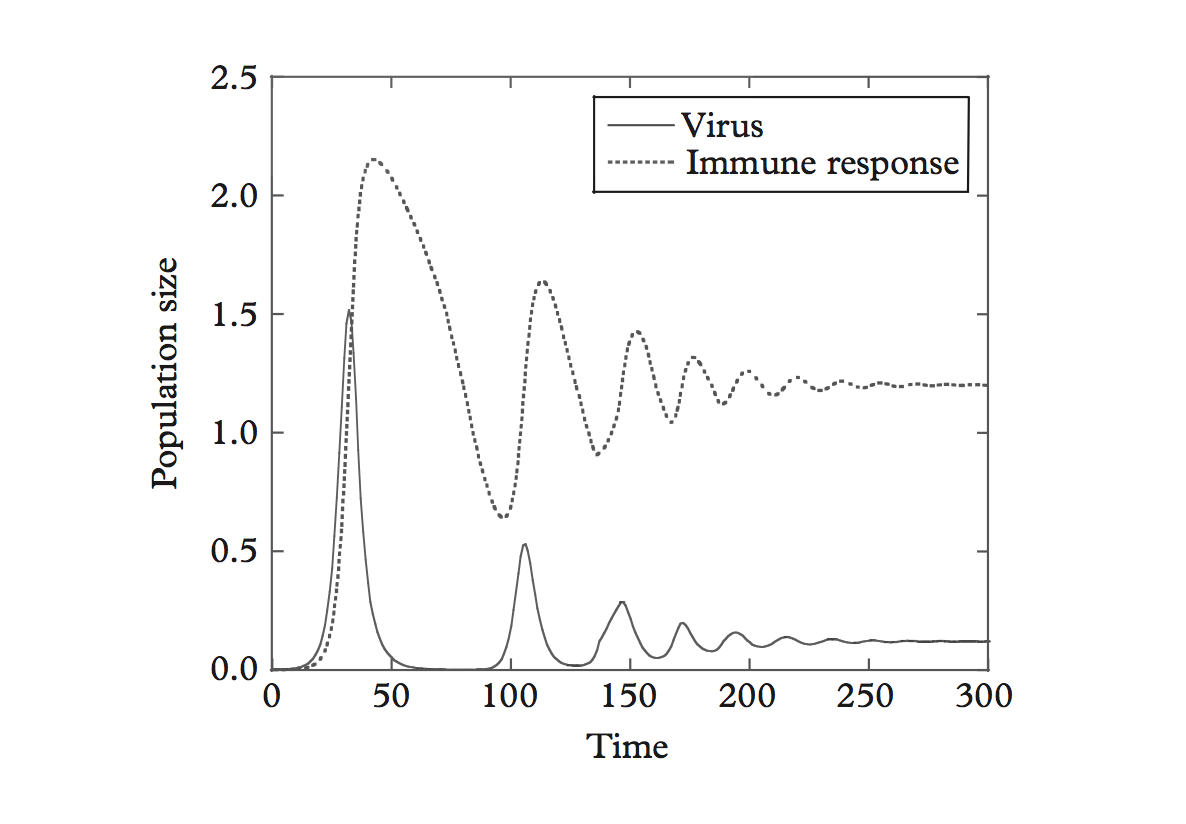
\includegraphics[scale=.4]{imgs/hiv_graph1.png}
    \label{fig:hiv1}
\end{figure}

\subsection{Modeling Our System with Multiple Viral Strains}
Suppose there are $N$ strains of the virus.  The $i$th strain of the virus $v_i$ and the immunal reaction $x_i$ to it can be modeled by the system of equations
\begin{equation}
    \begin{split}
        \dot v_i &= v_i(r - ax_i), \\
        \dot x_i &= -bx_i + cv_i
    \end{split}
\end{equation}
This adds a degree of randomness to our behavior as new viruses can appear at any point in time. Each new virus strain should result in a new immune response. Eventually a global immune response will take care of all $N$ viral strains regardless of mutation. This global response can be modeled by the system of equations
\begin{equation}
    \begin{split}
        \dot v_i &= v_i(r - ax_i - qz) \\
        \dot x_i &= -bx_i + cv_i \\
        \dot z &= kv - bz
    \end{split}
\end{equation}
Where $z$ is the cross reactive response that decays at rate $b$.  $v = \sum^{N}_{i=1} v_i$ is the total viral load. $q$ is the rate at which the virus evades the global response, $k$ is the rate at which the global response grows in comparison to the number of preheat viral strains.

\subsubsection{Getting Eigenvalues}

\begin{figure}[h!]
    \centering
    \caption{\textbf{\textit{Example of a cross-reactive immune response. The total population sizes of the viral load and the immune response are shown for r = 2.4, a = 2, b=0.1,c=1,q=2.4,k=1 with a random probability for the rise of new virus strains.}}}
    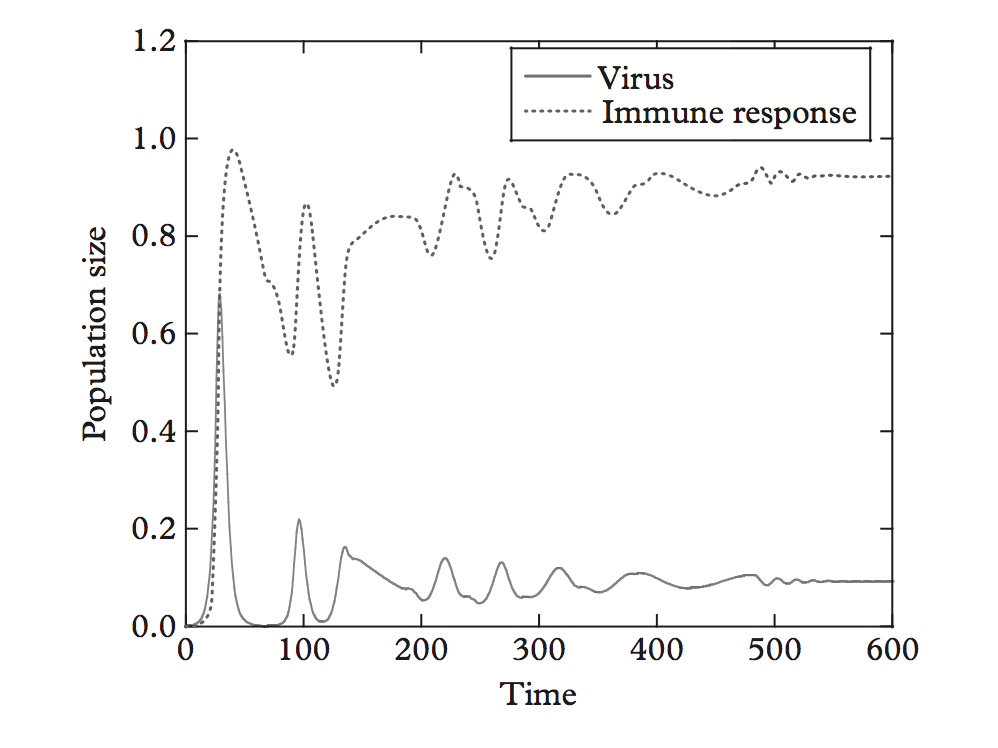
\includegraphics[scale=.4]{imgs/hiv_graph2.png}
    \label{fig:hiv2}
\end{figure}

\subsection{HIV Section}

\subsection{Ebola Section}

\section{Conclusion}
\label{sub:Conclusion}
Lorem ipsum dolor sit amet, id mea quidam pericula appellantur, ne quo vitae recteque. Duo ullum deserunt definitiones ea, ex has vocent constituam inciderint, at novum philosophia has. Summo facete audire eu pro, mazim tritani tibique ne quo. Justo deterruisset reprehendunt qui cu, nam te debet oblique incorrupte. Usu nominavi copiosae patrioque et, nec ferri constituto ei.



\begin{thebibliography}{9}
\bibitem{latexcompanion} 
Michel Goossens, Frank Mittelbach, and Alexander Samarin. 
\textit{The \LaTeX\ Companion}. 
Addison-Wesley, Reading, Massachusetts, 1993.
\end{thebibliography}


\end{document}
